% !TeX root = ../star_sporting_regulations.tex
% Add the above to each chapter to make compiling the PDF easier in some editors.

\newpage
{\bf Authors}
\\ \\Janis Mauch \emph{\\Founder of Student AirRace - Regulations Team \\janis.mauch@student-airrace.com}
\\ \\ Simon Pokorny \emph{\\Cofounder of Student AirRace - Technology Team \\simon.pokorny@student-airrace.com}
\\ \\ \\
{\bf Changelog}
\\ \\{\bf Current Version: \\Version Draft \getVersion{}}
\\ \\Previous Versions: \\ No previous Versions

\newpage
{\bf Preface}
\\ \\ Welcome to the Student AirRace competition! \\ \\
Get ready for an adrenaline-pumping experience as you showcase your talents and skills in the thrilling world of drone racing. 
For our team, this competition has been a dream come true, and we are honored to host it. 
At Student AirRace, our vision is to become the premier air race competition for students and one day, maybe even evolve into manned aircraft competitions.
\\ \\ 
Safety is our top priority, and we are dedicated to ensuring that all participants and spectators have a safe and unforgettable experience. 
We understand that the technology and regulations surrounding drones, eVTOLs, and UAS are constantly evolving, and we have done our best to create regulations that are comprehensive and up-to-date with the current state of the industry. 
However, we also understand that there is always room for improvement, and we welcome any feedback you may have to help us make this competition even better.
\\ \\ 
We have put a lot of hard work and dedication to get to this point and we can't wait to see what you have to bring to the table. 
We hope you will not only have fun, but also learn a lot and make valuable connections in the industry. 
Get ready to push your limits and soar to new heights as we witness the innovative solutions and ideas you will bring to the competition. 
Welcome to the racing of the future. You are now a part of it.
\\ \\ \\
Janis Mauch 
\\ \\Founder of Student AirRace

\newpage
{\bf What are the Sporting Regulations?} \\ \\
Welcome to the Sporting Regulations for the Student AirRace. This document outlines the rules and guidelines that govern the competition, with the goal of ensuring that all teams have a fair and safe experience. These regulations are separate from the Technical Regulations, which detail the specific requirements and standards for the design and construction of the unmanned aerial vehicles (UAVs) that will compete in the event.
\\ \\
The Sporting Regulations provide information on various aspects of the competition, such as the schedule of events, the scoring system, and the roles and responsibilities of the teams and organizers. Additionally, they describe the procedures for scrutineering, briefings, protests, and other important activities that occur before, during, and after the competition.
\\ \\
It is important that all teams carefully read and understand both the Sporting Regulations and Technical Regulations in order to ensure that their UAVs meet the necessary requirements and that they are fully prepared for the competition. Any questions or concerns regarding these regulations can be directed to the organizers for clarification.
\\ \\
If you were looking for the technical regulations governing the construction and specifications of the participating UAVs, they can be found on our website at www.student-airrace.com/competition. These regulations should be read in conjunction with the sporting regulations provided in this document.

\newpage
{\bf Notes:
\begin{itemize}
  \item Contents marked in \textcolor{red}{red} are still subject to change and should be seen as current estimations and placeholders.
  \item This whole document is still a work in progress. Some points may still be left empty.
  \item If you have any comments on specific regulations, for example, think that they are not required, are too strict or don't make sense, don't hesitate to contact regulations@student-airrace.com.
\end{itemize}
}
\hspace{10mm}

{\bf Abbrevations:}
\begin{tabbing}
  {\bf AI~~~~~~~~~~~~~~} \= Artificial Inteligence
  \\{\bf ARP} \> Aeronautical Recommended Practices
  \\{\bf CE} \> Conformité Européene (European Conformity)
  \\{\bf DC} \> Direct Current
  \\{\bf EASA} \> European Union Aviation Safety Agency
  \\{\bf e-ID} \> electronic identification
  \\{\bf EU} \> European Union
  \\{\bf EU-LBT} \> EU Listen Before Talk
  \\{\bf EIRP} \> Equivalent Isotropically Radiated Power
  \\{\bf ESC} \> Electronic Speed Controller
  \\{\bf EUROCAE} \> European Organisation for Civil Aviation Equipment
  \\{\bf FPV} \> First Person View
  \\{\bf HITL} \> Hardware-in-the-loop
  \\{\bf ICAO} \> International Civil Aviation Organization
  \\{\bf ISO} \> International Organization for Standardization
  \\{\bf Lipo} \> Lithium Polymer
  \\{\bf LTE} \> Long-term Evolution
  \\{\bf MTOW} \> Maximum Take-Off Weight
  \\{\bf NOTAMS} \> Notice to Airmissions
  \\{\bf RC} \> Remote Control
  \\{\bf RTH} \> Return to Home
  \\{\bf SORA} \> Standard Operating Risk Assessment
  \\{\bf UAS} \> Unmanned Aerial System
  \\{\bf UAV} \> Unmanned Aerial Vehicle
\end{tabbing}




\newpage

\newpage

 \section{Competition Outlines}
  
\subsection{Objective of the competition}
   \begin{enumerate}
      \item \emph{What are our values? What is the ultimate goal of the competition? What do we want to achieve?}
    \end{enumerate}


    \subsection{Participants}
    \begin{enumerate}
      \item Only enrolled university (or of comparable institutes) students are allowed to actively take part in the competition.
      \item If a team member has graduated during six months before the competition, they may still participate.
      \item If a team member has graduated during the eighteen (18) months before the competition and has played a significant role within the team,
      the team may send an application to the organizer, requesting their participation. 
      \item Students attending other universities which are within a reasonable distance of a participants university (e.g. in the same city) may join
      a student team from said university.
      \item If a students university already has a competing team, the student is not allowed to join a competing team of 
      another university.  
      \item The team size is not limited to a maximum number of members. However the organizer may limit the of allowed on site participants to a maximum of \textcolor{red}{15} for each team at the final event.
      \item PHD candidates who are still enrolled or working for the university are allowed to join the teams. 
    \end{enumerate}

    \subsection{Competition Rewards}
    \begin{center}
        \begin{tabular}{|c|c|c|} 
          \hline
          Position & Dicipline & \textcolor{red}{Moneytary Award} \\
          \hline
          1st & Overall & \textcolor{red}{25\%} \\ 
          \hline
          2nd  & Overall & \textcolor{red}{15\%} \\ 
          \hline
          3rd & Overall & \textcolor{red}{10\%} \\ 
          \hline
          1st & AI racing & \textcolor{red}{15\%} \\ 
          \hline
          2nd  & AI racing & \textcolor{red}{9\%} \\ 
          \hline
          3rd & AI racing & \textcolor{red}{6\%} \\ 
          \hline
          1st & Safety & \textcolor{red}{5\%} \\ 
          \hline
          1st & Design Maturity & \textcolor{red}{5\%} \\ 
          \hline
          1st & Innovation and Sustainability & \textcolor{red}{5\%} \\ 
          \hline
          1st & Special Prize & \textcolor{red}{5\%} \\ 
          \hline
        \end{tabular}
      \end{center}
      

    \begin{enumerate}
      \item Every winner of one of the categories mentioned above will receive the following prizes:
      
      \begin{itemize}
        \item Trophy according to their position and discipline
        \item Free entry to the competition in the next year.
        \item Special prizes like tours etc. by sponsors
        \item \textcolor{red}{Prize Money according to the table}
      \end{itemize}

      \item \textcolor{red}{There is currently no prize money planned for the competition. Since the registration fee is only intended as a way of giving an incentives to the teams to actually compete the registrations fees might get split up between the winning teams. \\ \\ Furthermore Student AirRace is looking into 
      the possiblity of collecting further money as potential prize money for the teams. If the option for prize money is agreed upon, then it would be split according to the percentages in the table above. }
    \end{enumerate}

    \newpage
    \section{Competition Processes}

    \begin{figure}[h!]
      \centering
       \IfFileExists{figures/NavigateStudentAirrace.png}{%
       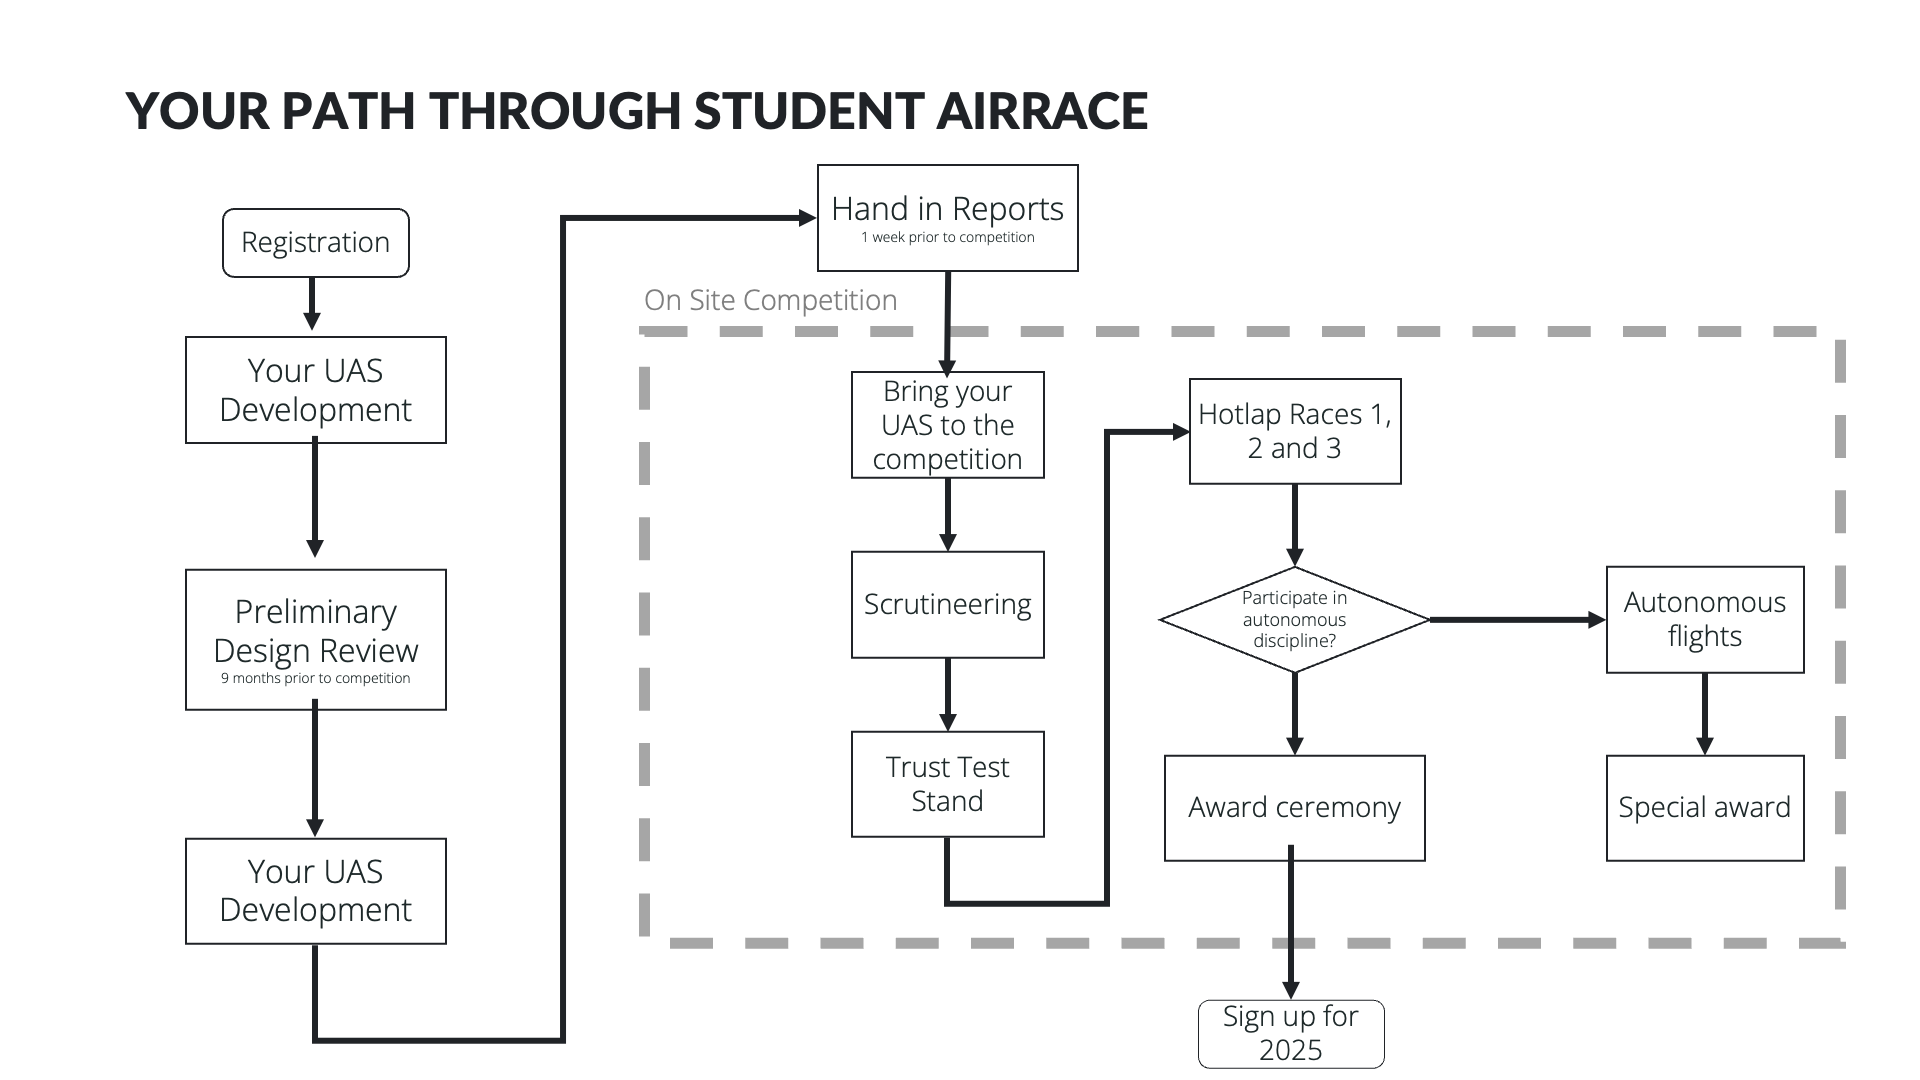
\includegraphics[height=100mm]{figures/NavigateStudentAirrace.png}
       
       }{%
       \vspace*{100mm}
       }
     \caption{\textit{This flowchart illustrates the registration processes and mandatory events for the competition.}}
     \end{figure}

    \subsection{Registration Process}
    \begin{enumerate}
      \item Teams can register for the competition on the website of Student AirRace. The sign up page can be found at www.student-airrace.com/recruiting 
      \item Only one team per individual university may register for the competition.  
      \item The participating teams will be chosen by the organizer. This will partly happen on a "First Come First Served"-Base but also
      on the perception and opinion of the organizers whether a team will be able to meet the requirements and standards of the competition. 
    \end{enumerate}

    \subsection{Later Changes to the Registration}
    \begin{enumerate}
      \item Teams may sumbit changes to the information they have provided in their registration up to six months before the competition. This enables to teams to rebrand or change their starting numbers.
      \item If in the opinion of the organizer, a competitor is likely to not meet the requirements or standards
      of the competition, they are allowed to reject them after the registration process. 
      \item In case of withdrawal from the competition, the team must notify the oganizers as soon as possible. Withdrawals must be entered until six months before the competition. 
      Any non-existing or later withdrawals may be penalized by the organizers with point deduction or ban from future events. 
    \end{enumerate}

    \subsubsection{Participation Fee}

    \begin{enumerate}
    \item A participation fee of \textcolor{red}{300 \euro{}} per team will be required to participate in the competition.
    \item The fee will go into the prize money pool and will be distributed to the participating teams according to the prize money table, which will be determined by the organizers.
    \item The fee is required as a sort of deposit to ensure the team's commitment to the competition and their timely arrival.
    \item The payment of the fee is due after \textcolor{red}{6 months} after registration and will be handled by the organizers.
    \item Teams who fail to pay the participation fee will not be allowed to participate in the competition.
    \end{enumerate}

    \subsection{Expenses}
    \begin{enumerate}
      \item The organizers will not support or reimburse the teams for travel, accommodation or any other expenses. 
      \item The competitors may search for private, university or company sponsors to cover any of their expenses.
    \end{enumerate}

    \section{Competitor Organization}

    \subsection{Just Culture}
    \begin{enumerate}
      \item The teams and the organizer commit to adopting a so called "Just Culture". This is important to ensure the safety of the competition and its participants.
      \item The team leaders commit themselves to learning about Just Culture and to educate their team members about it.
      \item Participants who notice safety related issues in their team or within the competition are able to report them anonymously  to info@student-airrace.com. This will not bear any
      negative consequences for them nor their team. 
      \item \textcolor{red}{Student AirRace is also seeking to provide the teams with workshops about this topic.}
    \end{enumerate}

    \section{Practice during development}
    \begin{enumerate}
      \item During development, testing practice of their UAVs the teams are required to meet all the laws and requirements of their flight location. 
      \item There is no maximum limit on how much time the teams invest into flying before the competition. However a minimum flight experience on the competititon UAV and for the pilots must be documented. More can be found at Section \ref{pilotrequirements}
    \end{enumerate}

    \subsection{Team Documentation}
    The following rules are not meant as a way of annoying the teams or making their lives hard. The competitions success is in the hands of the competitors. In order to grow the competition 
    in a sustainable manner we need to keep certain aviation and safety standards. Furthermore those rules are supposed to teach you standard aviation processes and help you learn and grow. 
    In case you have any questions on how to approach those flight documents, the organizing team of Student AirRace will gladly assist you. Safety and the success of this competition is in all of our hands.
    \begin{enumerate}
      \item The teams are required to document all flights conducted with their prototypes in physical and/or digital flight books. They must note at least location, flight time, pilot flying 
      as well as observations, abnormal events or incidents during the flight.
      \item The teams are required to document their pilots personal flights and flight time on aircrafts comparable to or on the competition aircraft (e.g. Racing Quadrocopters)
      for each individual flight and in a cumulative manner. These documents will be checked according to \ref{pilotrequirements} at the competition. 
      \item The teams must keep up to date records about the equipment installed on the UAV. This includes all electronic and mechanical subassemblies on the UAV. 
      Changes must be clearly marked and recorded. 
      \item Teams are required to keep up to date records of any damages or problems on the UAV. Even if the aircraft might still be flightworthy. 
      Any repairs will have to be documented, stating the reason of the repair and a short overview of the process of the repair. 
    \end{enumerate}

    \subsection{Feedback for the organizer}
    \begin{enumerate}
      \item The teams are asked to inform the organizers about any obstacles or issues they run into, which might be caused by
      too strict or too lenient regulations. The organizers will gladly receive any feedback and integrate it into the regulations. 
      \item Teams are required to inform the organizers about any incidents, which lead to loss of the UAV, damage to ground structures, injury, or death. 
    \end{enumerate}



    \section{Final Competition Logistics}
    \subsection{Logistics}
    \begin{enumerate}
      \item Each team can ship a maximum of one twenty (20) ft shipping container to the location of the competition beforehand. The container will be placed right next to the teams reserved location in the paddock.
      \item The teams are responsible for shipping expenses and on time delivery of the containers. Shipping of the containers is possible from \textcolor{red}{three months }before the final competition takes place.
      \item The organizers will not accept any other types of shipment unless different agreements are in place beforehand.
    \end{enumerate}

    \subsection{Paddock}
    \begin{enumerate}
      \item The paddock is where the teams are allowed to work on their UAS. 
      \item Each team gets their own spot "Team Home" within the paddock (ca. 7m x 7m) where they can put up a small tent, flags etc. Their shipped containers will also be right next to their spot. 
      \item Under no circumstances may any UAS fly within the paddock without prior approval by the organizer. This will lead to heavy penalties up to disqualification. 
      \item The organizer will provide the teams with power within their team home.    
    \end{enumerate}


    \section{Final Competition Organization}

    \subsection{Scrutineering}

    \begin{enumerate}
    \item The purpose of the scrutineering process is to ensure that all vehicles comply with the regulations set forth by the organizers and will take place before the Thrust Test Stand Event.    \item Each team will be assigned a specific time slot for scrutineering, which will be communicated to them in advance.
    \item If a team fails to attend their assigned scrutineering time slot, they may be penalized or disqualified.
    \item The penalties for non-compliance may range from minor point deductions to disqualification from the competition, depending on the severity of the infraction.
    \item The organizers may use different checks for each vehicle, based on the unique features and design of the vehicle.
    \item Examples of checks that may be conducted during scrutineering include, but are not limited to:
    \begin{itemize}
    \item Weight checks
    \item Size measurements 
    \item Electrical system checks
    \item Structural integrity checks
    \item Safety system checks
    \item Paperwork, flightbook and insurance check
    \end{itemize}
    \item Teams are responsible for ensuring that their vehicle is fully functional and ready for scrutineering. Any repairs or adjustments required must be made prior to the scheduled scrutineering time slot.
    \item If a team fails scrutineering, they will be given a specific period of time in which to rectify the issue and return for re-inspection. If they are unable to rectify the issue within the allotted time, they may be penalized or disqualified.
    \end{enumerate}

    \subsection{Team Briefings}
    \begin{enumerate}
      \item At each day of the competition, there will be a team briefing.
      \item For specific roles, such as pilots there may be additional mandatory briefings.
      \item Each team briefing must be attended by the team members which will be present at the flightsite during the flights to the briefing.
      \item One point can be deducted by the organizer for each member which is missing during the briefings.
    \end{enumerate}

    \subsection{Parc Fermé}
    \begin{enumerate}
      \item Parc Fermé begins at the moment the Team starts the Thrust-Stand-Event for the first time during the competition days. It ends with the completion of all three competition flights. 
      \item While Parc Fermeé is active teams are not allowed to work on the UAVs. Only the following works are allowed to be carried out: 
      \begin{itemize}
        \item Balancing of propellers
        \item Cleaning of any parts of the aircraft
        \item Exchange of batteries for a 1:1 replacement
        \item Charging of batteries 
        \item Reading logs and taking measurements
        \item Tightening of any loose screws
        \item Adjustment of minor software parameters. 
        \item Repair of accident damage and 1:1 replacement of broken parts as long as the crash is deemed by the organizer to not have happened on purpose. 
      \end{itemize}
      \item Work on safety related systems may be done after submitting a written request to the organizer and getting it accepted by the organizer. 
    \end{enumerate}

    \subsection{Protests}
    \begin{enumerate}
      \item Teams are allowed to launch a protest against any decisions, rules or penalties imposed by the organizer.
      \item They must do so within 6 hours of the decision. 
      \item The protest must be sent to the organizer in written form, this can happen digitally. It must state the decision, the reason for protest and contacts from the team.
      \item Along with the protest the team will be deducted 10 Points from their final score. If the organizers agree with the protest, the teams receive those points back. 
    \end{enumerate}

    \section{Preliminary Design Review (PDR)}
    \begin{enumerate}
    \item The PDR is conducted approximately nine (9) months prior to the event.
    \item The purpose of the PDR is to ensure that the teams are on track with their development and that their aircraft meets the rules of the competition.
    \item The appointment for the PDR is made together with the teams and must be attended by the responsible team leads.
    \item During the PDR, the organizers will review the teams' progress and may ask questions to ensure that the teams understand the rules and have a clear path forward in their development.
    \item The PDR is meant to be a support for the teams and not a way to tease or disqualify them.
    \item The PDR is mandatory and failure to attend may result in penalties or disqualification from the competition.
    \item The teams are required to provide the following documentation for the PDR:
    \begin{itemize}
    \item A detailed design report that includes the concept, system design, subsystems, and components.
    \item A preliminary analysis of the flight performance, including the expected thrust-to-weight ratio, endurance, and speed.
    \item A preliminary risk assessment and safety analysis.
    \item A detailed description of the UAV's control and navigation systems.
    \item A list of all components used, including the specifications and supplier information.
    \end{itemize}
    \item The PDR documentation must be submitted to the organizers at least two (2) weeks prior to the scheduled PDR appointment.
    \item The PDR will be conducted remotely, via video conference or other means as determined by the organizers.
    \end{enumerate}


    \section{Reports}

    \subsection{Design Maturity and Technical Report}
    \subsubsection{Technical Report}
    \begin{enumerate}
    \item Each team must submit a technical report before the start of the competition that outlines the technical details of their drone.
    \item The technical report must be submitted no later than 7 days prior to the competition. The exact deadline for submission will be announced to the teams in advance. Failure to submit the safety report by the deadline may result in penalties or disqualification at the discretion of the jury. It is the responsibility of each team to ensure timely submission of the safety report to avoid any adverse consequences.
    \item The technical report must include details such as the drone's weight, dimensions, power source, flight time, range, maximum speed, and any other technical specifications required by the organizers.
    \item The technical report must also include information about the drone's control system, sensors, communication systems, and any other relevant components or subsystems.
    \item The technical report must be a maximum of 10 pages long, written in English, and submitted in PDF format.
    \item The technical report will be graded by a jury and is worth a maximum of 15 points.
    \item The jury will evaluate the technical report based on the level of detail provided, the quality of the engineering and design work, and the overall technical feasibility of the drone.
    \item Teams may use the technical report as an opportunity to highlight any innovative or unique features of their drone's design or technology.
    \item The technical report may also be used by the jury to determine whether a team is eligible to participate in the competition or to determine penalties or disqualifications for technical violations during the competition.
    \end{enumerate}
    
    \subsubsection{Design Maturity}
    \begin{enumerate}
    \item Each team's drone must meet minimum standards of design maturity to be eligible for participation in the competition.
    \item The drone's physical construction must be of professional quality and meet acceptable aviation standards. This includes no hanging cables, proper soldering, and proper engineering practices.
    \item The team must demonstrate a high level of care and attention to detail in the construction and presentation of their drone.
    \item The design maturity evaluation will be worth a maximum of 15 points and will be based on the quality of the drone's construction and presentation.
    \item The jury may evaluate the design maturity of the drone at any point during the competition and may disqualify any team whose drone does not meet minimum design maturity standards.
    \end{enumerate}
    
    
    
    
    \subsection{Innovation and Sustainability Report}
    The innovation and sustainability report is an opportunity for teams to demonstrate their commitment to sustainable innovation, and to showcase the potential of their drone's features for promoting sustainability in aviation.
    \begin{enumerate}
    \item Each team must submit an innovation and sustainability report before the start of the competition that outlines the innovative and sustainable features of their drone.
    \item The innovation and sustainability report must be submitted no later than 7 days prior to the competition. The exact deadline for submission will be announced to the teams in advance. Failure to submit the safety report by the deadline may result in penalties or disqualification at the discretion of the jury. It is the responsibility of each team to ensure timely submission of the safety report to avoid any adverse consequences.
    \item The innovation and sustainability report must include details such as how the team's drone uses sustainable materials, energy-efficient systems, or innovative features to solve a real-world problem.
    \item The innovation and sustainability report must be a maximum of 15 pages long, written in English, and submitted in PDF format.
    \item The innovation and sustainability report will be graded by a jury and is worth a maximum of 25 points.
    \item The jury will evaluate the innovation and sustainability report based on the level of detail provided, the originality and creativity of the team's approach, and the potential impact of the drone's features on sustainability or innovation.
    \end{enumerate}
    
    \subsection{Safety Report}
    Safety is the top priority of Student AirRace. Teams must submit a safety report detailing their drone's safety features, procedures, and pilot training. The report helps teams identify and mitigate safety risks and highlight safety features. The jury evaluates the report to determine eligibility and penalties for safety violations.
    \begin{enumerate}
    \item Each team must submit a safety report before the start of the competition that outlines the safety features and procedures of their drone.
    \item The safety report is a crucial aspect of the competition and is taken very seriously. Failure to submit a safety report, or failure to provide a thorough and accurate report, may result in penalties or disqualification. It is important for teams to prioritize safety and take the safety report seriously to ensure the safety of all participants and spectators.
    \item The safety report must be submitted no later than 7 days prior to the competition. The exact deadline for submission will be announced to the teams in advance. Failure to submit the safety report by the deadline may result in penalties or disqualification at the discretion of the jury. It is the responsibility of each team to ensure timely submission of the safety report to avoid any adverse consequences.
    \item The safety report may include details such as how the team's drone ensures the safety of the pilot, spectators, and other aircraft in the area.
    \item The safety report may be a maximum of 20 pages long, written in English, and submitted in PDF format.
    \item The safety report will be graded by a jury and is worth a maximum of 25 points.
    \item The jury may evaluate the safety report based on the level of detail provided, the effectiveness of the safety features and procedures, and the overall safety of the drone and its operation.
    \item The safety report may also include details about the team's pilot training and qualifications, as well as the training and qualifications of any personnel involved in the drone's operation or maintenance.
    \item The team may also provide information about any redundancy features of the drone, such as redundant power sources or communication systems.
    \item The safety report may detail the total number of flight hours completed by the drone and any previous crashes or incidents, along with the lessons learned from those incidents and any changes made to improve safety.
    \item Teams may also use the safety report as an opportunity to highlight any safety features or procedures that may impact the drone's performance negatively, but which provide a significant increase in safety.
    \item The jury will evaluate the safety report based on how well the team is able to demonstrate their commitment to safety and their ability to identify and mitigate potential safety risks.
    \item The safety report may be used by the jury to determine whether a team is eligible to participate in the competition, or to determine whether any penalties or disqualifications may be warranted in the event of a safety violation during the competition.
    \end{enumerate}

    \section{Final Competition Disciplines}
    \subsection{Mandatory Disciplines}

    \subsubsection{Scoring}
    \begin{enumerate}
      \item Each team must compete in each of the mandatory disciplines, mentioned below. 
      \item A team can achieve a maximum of twohundredeleven (155) points which can be collected during different mandatory events.
      \item At the end of the competition and after the deduction of any penalties, the team with the most cumulated points is declared as the winner of the main event. 
      \item If two teams achieve the exact same amount of points, also known as a dead heat, after all points have been awarded the winner will be declared by who has scored more points in the safety report. 
      If both of them have also equally scored equally in this discipline this process repeats for the Technical Report, design maturity and innovation \& sustainability disciplines in the hereby mentioned order. If this doesn't deliver any result the organizer will make a decision. 
      \item The following table shows how the total points are distributed across the individual disciplines. 

      \begin{center}
        \begin{tabular}{|c|c|c|} 
          \hline
          Discipline & Points & Awardment Process \\ 
          \hline
          Hotlap Races & 75 & Time measured by organizer \\ 
          \hline
          Safety & 25 & Jury Decision \\ 
          \hline
          Design Maturity and Technical Report & 30 & Jury Decision \\ 
          \hline
          Innovation and sustainability & 25 & Jury Decision \\ 
          \hline
        \end{tabular}
      \end{center}
    \end{enumerate}

    \subsection{Comparability between runs}
    \begin{enumerate}
      \item To ensure comparability between the runs, the organizers are going to set limits on the metrological conditions during which the runs can happen. If the organizer is calling the conditions to be fine for takeoff the takeoff time window rule applies. \\
      The organizers will monitor the following conditions at the track during the flights:
      \begin{itemize}
        \item Precipitation
        \item Temperature 
        \item Windspeed
        \item Humidity
        \item Air Pressure
        \item GNSS Connectivity and satellite number at fixed position on site (GPS only) 
        \item Frequency jamming
      \end{itemize}
    \end{enumerate}

    \subsection{Race Course Layouts}
    \begin{enumerate}
      \item The Race course layout will be build within a rectengular shaped zone. This rectangle has sidelengths of 1500m and 500m. The maximum height during the flight is limited to 100m Above Ground (AGL).
      \item No point within the race course layout is going to be further away than 1000m from the Ground Station. Also every point of the racecourse layout will be able to be flown within Line Of Sight of the Ground Station. 
      \item Race courses consist of an assembly of different predetermined race course elements which are published with the regulations.
      \item The official assembly of race course layouts for the three hotlap sessions will not be published until shortly before the competition, in order to prevent the teams from overfitting their aircraft to one specificn racecourse. 
      \item Race course assembly kits are published in Annex A. 
      \item The race courses are marked with the help of 12m high pylons or flags. 
    \end{enumerate}


    \section{Flight Operations at the final competition}
    \begin{enumerate}
      \item During the flights, the teams must assign different roles within the team at the track, which are defined in the latter regulations.
      \item Each person which fullfills a required role must be able to fluently communicate to the organizers in english.
      \item A minimum of four (4) persons are required at the track to be allowed to conduct the flights.
      \item A maximum of ten (10) persons by a team are allowed at the track. For clarification: This does not affect the amount of persons each team is allowed to have in the paddock.  
    \end{enumerate}

    \subsection{Required roles during Flight}
    \begin{enumerate}
      \item \textbf{PL: Pilot}\\The pilot is the person responsible for flying the UAV.
      \item \textbf{AO: Airspace Observer/Spotter}\\The AO stands next to the PL and has an unobstructed view of the airspace around the drone. They talk to the PL directly in person. The PL and AO are allowed to communicate via intercom if they stay right next to each other. 
      \item \textbf{FE: Safety Engineer}\\The safety engineer is the one who was responsible for the safety report. Their task is to constantly monitor the situation and warn the others if they are getting into any problematic situations. 
      \item \textbf{FOL: Flight Operations Lead}\\The FOL makes the tactical decisions during the flight. They request for Takeoff Permission from CL (Competition Lead). They manage contingency and emergency procedures. They are essentially the boss of the teams operation.
      \item All of the roles and the names of the responsible team members, as well as backup per position will need to be entered to the organizer 30 days prior to the competition. 
    \end{enumerate}


    \subsection{Requirements for the pilots}\label{pilotrequirements}
    \begin{enumerate}
      \item Each team must have at least three different designated pilots. The names of those pilots must be sent to the organizer at least 
      30 days before the competition. 
      \item Each pilot must have flown and documented at least twenty (20) hours on comparable UAVs (e.g. Racing Quadrocopters) in the past 12 months.  
      \item The pilots must be able to fluently communicate with the organizers in English, in order to be able to follow safety relevant commands during flight.
      \item The pilots may have have to perform a flight test check in front of the organizers at the competition. This is just a quick test flight with any multicopter UAS to demonstrate the pilots basic flight skills.
    \end{enumerate}




    \section{Disciplines}
    \subsection{Thrust Test Stand}
    \textbf{Disciple Outline}
    The thrust test stand is a crucial part of the Scrutineering process and ensures that teams meet all the necessary requirements outlined in the technical regulations. It also serves as a means for organizers to assess the safety and reliability of the teams' vehicles and their technical condition. A successful performance in this discipline is required to qualify for takeoff clearance for the Hotlap races.
    \begin{itemize}
      \item Each team must demonstrate their vehicle's performance on the thrust test stand.
      \item Each team will be assigned a specific time for their vehicle to be tested and must be ready at that time.
      \item The vehicle must be mounted on the thrust test stand using the adapter specified in the technical regulations.
      \item The team must run their vehicle for at least 50\% of their battery capacity on the thrust test stand.
      \item The shape of the used thrust curve over time is at the discretion of the competitors.
      \item The team must complete the thrust test stand event within 15 minutes. Failing to do so or not utilizing at least 50\% of the battery capacity will result in a penalty.
      \item The Thrust to Weight Ratio (TWR) of the vehicle, calculated from its weight during scrutineering, must be at least 2:1. The minimum Thrust measured on the vehicle Thrust Test Stand must exceed the required value to achieve this ratio for at least 5 seconds under standard atmospheric conditions.
      \item If the atmospheric conditions during testing do not meet the ICAO standard atmosphere conditions, a correction factor based on the current air density will be applied to the thrust stand results linearly.
      \item The teams are responsible for securing their aircraft on the thrust test stand.
      \end{itemize}



    \subsection{Hotlap races}
    \textbf{Disciple Outline}
    \begin{itemize}
      \item There will be a total of three (3) hotlap races on different tracks during the competition. The following rules apply to a single race.
      \item Each team will be given a \textcolor{red}{fivteen (15) } minute time window during which they can conduct their flights. 
      \item Each team is only allowed to set a maximum of five timed (5) laps during their time window. 
      \item Each laptime will be logged by the organizer. It counts as the time from which the aircraft passes the start/timing line until the aircraft has crossed the timing/finish line. 
      \item The points will be awarded in order of fastest hotlap achieved by each of the teams during their time window.
    \end{itemize}

    \subsubsection{Hotlap Race Rules}
    \begin{enumerate}
      \item The following rules apply in combination with the later specified Race Procedures.
      \item The lap time will be recorded according to the Hotlap Race Procedures outlined in the following Race Procedure sections.
      \item Teams are required to pass through every gate on the course. Missing a gate will result in the lap time being invalidated.
      \item If a gate is defined as a pole, teams must pass the pole on the side specified by the organizers. Failing to do so will result in the lap time being invalidated.
      \item Teams must ensure their drones remain within the flight perimeter, or geocage, at all times. Any drone found to be flying outside the geocage may be disqualified or face penalties.
      \item Each drone will be able to fly their hotlap individually, with no other drones operating simultaneously. This is to ensure safety and avoid interference during the race.
      \item The start gate can be crossed at any velocity. Teams are allowed to have a run-up, provided it does not exceed the boundaries of the location.
      \item A lap can be aborted at any time at the team's discretion. If a lap is aborted, the time will be reset and will start again once the team's drone crosses the start gate for a new lap.
      \item Each team is allowed to pass through the start gate for a total of five times. However, they may conduct practice laps without crossing the start gate.  
      \item The points will be awarded in order of fastest hotlap achieved by each of the teams during their time window. Only the fastest lap of the competitor will be counted. Even if their second fastest lap should be faster than the one of another compeitor.
      \item If two or more competitors achieve the exact same finish time, their points will be added together and divided equally across the them.  
      \item Teams are expected to follow all additional rules and guidelines provided by the organizers. Dangerous flying will immediately result in disqualification. 
      \item During the hotlap time window no one is allowed to touch the UAV withot prior authorization by the organizers. If any member of the competing team touches the drone, it will result in immediate disqualification.
    \end{enumerate}


    \subsubsection{Hotlap Race Procedures}
    \textbf{Start of a Hotlap Race}
    \begin{enumerate}
      \item Each team gets a certain time slot during which they are allowed to conduct their hotlaps. 
      \item The organizer will ensure that the time is only started if a set of weather conditions is met. Afterwards there is no going back. This is comparable to the process ski jumpers undergo during their competitions.
      \item The start of the session is called by the organizer. Afterfwards the clock is started and a \textcolor{red}{fivteen (15)} minute timer begins to tick down. The teams must conduct their hot laps within this time frame.
      \item The teams are free to conduct flights however they'd like to during this time as long as all other rules are adhered to. This is up to their strategy. One team may fly three slow training laps and one racelap. Another team may set three race times or wait on the ground for exactly the right wind conditions.
    \end{enumerate}
    \textbf{Suspension of a Hotlap Race}
    \begin{enumerate}[resume]
      \item The session can be suspended by the organizer in case of unexpected events such as uninvolved people or aircraft entering the flight test area. A sudden change of weather which exceeds the limits set by the organizer may also lead to a suspesion of the session. 
      \item In case of a suspension the clock will be stopped. 
      \item The pilot must abort the lap immediately and slow the UAS down. Further actions will be coordinated together with the organizers depending on the situation.
      \item The pilot must stay away as far as possible from uninvolved people as possible at any point in time. 
    \end{enumerate}

    \textbf{Resumption after suspension of a Hotlap Race}
    \begin{enumerate}[resume]
      \item The clock is started from where it was stopped beforehand.
      \item Depending on the situation the organizers may add additional time to the clock, and/or allow the competitior to charge their battery to a certain level in order to compensate for the suspension.
    \end{enumerate}

    \textbf{Finish of a Hotlap Race}
    \begin{enumerate}[resume]
      \item The finish of a session is called after the fivteen (15) minute time window is over. After this the teams are not allowed to start a new lap.
      \item Teams may finish the current lap in progess if it does not take longer than two minutes.
      \item Teams may communicate their wish to prematurely end the current Hotlaprace to the organizer. For example if there's still time left but the battery charge is not enough to conduct another safe lap.
      \item In case of a ground colission from which the team is not able to safely recover the session is also ended. 
      \item The organizer may call an early end for a session if they deem a contiuation of the flight as unsafe. The session will not be retaken.  
      \item If the team doesn't manage to land at the landing pad, even though a safe landing is possible after the end of the race a penatly is applied by the organizers.
    \end{enumerate}

 

    \subsection{Autonomous Races}
    \textbf{Disciple Outline: }The autonomous races will test the ability of the teams to develop and implement autonomous control algorithms for their drones. These races will be held on a separate track and will have their own set of rules. THIS DISCIPLINE IS NOT MANDATORY.
 
    
    \begin{itemize}
      \item There will be a total of three (3) autonomous hotlap races on different tracks during the competition. The following rules apply to a single race.
      \item Each team will be given a \textcolor{red}{fivteen (15) } minute time window during which they can conduct their flights. 
      \item Each team is only allowed to set a maximum of five timed (5) laps during their time window. 
      \item Each laptime will be logged by the organizer. It counts as the time from which the aircraft passes the start/timing line until the aircraft has crossed the timing/finish line. 
      \item The points will be awarded in order of fastest autonomous hotlap achieved by each of the teams during their time window.
    \end{itemize}


    \subsubsection{Autnomous Race Rules}
    \begin{enumerate}
    \item The following rules apply in combination with the later specified Autnomous Race Procedures.
    \item Each team must design and program their own autonomous control algorithms for their drones.
    \item Teams may choose to build a new second drone specifically for the autonomous races, as long as it meets all the technical regulations outlined in the technical regulations.
    \item Alternatively, teams may use the same drone for both the manual and autonomous disciplines.
    \item All calculations for autonomous control algorithms must be run onboard the drone and cannot be executed from a ground station or other external computing device.
    \item The drone may communicate with external devices for the purpose of receiving location data or other necessary information, but all control and decision-making processes must be performed onboard the drone.
    \item Each lap must be completed autonomously by the drone without a single intervention by a human. Otherwise the lap will be invalidated.
    \item The drones must pass through every gate on the course. Missing a gate will result in a time penalty.
    \item If a gate is defined as a pole, drones must pass the pole on the side specified by the organizers. Failing to do so will result in a time penalty.
    \item Drones must remain within the flight perimeter, or geocage, at all times. Any drone found to be flying outside the geocage may be disqualified or face penalties.
    \item The start gate can be crossed at any velocity. Teams are allowed to have a run-up, provided it does not exceed the boundaries of the location.
    \item The points will be awarded in order of fastest lap achieved by each of the teams during the race.
    \item If two or more competitors achieve the exact same finish time, their points will be added together and divided equally across them.
    \item Teams are expected to follow all additional rules and guidelines provided by the organizers. Dangerous flying are having no clear intend to properly fly the laps will immediately result in disqualification.
    \end{enumerate}

    \subsubsection{Manual Control, Safety Functions, and Autonomous Flight}
    \begin{enumerate}[resume]
    \item The drone used in the autonomous race must be capable of both manual control and autonomous flight.
    \item All drones used in the autonomous races must also be able to be manually controlled by the team and always manually overwritable.
    \item A safety pilot must be in place to take over the drone by manual control.
    \item The drone must have the capability of triggering safety functions such as kill switches and Return to Home (RTH) capabilities.
    \item The team must be able to trigger these safety functions at any time during the race if necessary.
    \item The drone must be presented to the scrutineering committee prior to the start of the autonomous race to ensure that it meets all manual control, safety function, autonomous flight requirements and the technical regulations.
    \item The team may use manual flight to move the drone to the designated starting position or landing spot before the race begins, or to interfere with the drone during the race if necessary for safety reasons or to abort/restart a lap.
    \item Once the race begins at the start gate, the drone must autonomously fly the course without any further manual flight input.
    \item Any manual flight input between the start gate and finish gate that affects the drone's flight path or speed will result in an invalid lap time.
    \item The team may be allowed to retake the lap if the manual flight input was due to safety reasons and was not the fault of the team.
    \item Violation of the rules regarding manual control, safety functions, and autonomous flight may result in disqualification.
    \end{enumerate}





    \subsubsection{Race Procedures}
    \textbf{Start of the Autonomous Race}
    \begin{enumerate}
    \item Each team will be given a \textcolor{red}{fivteen (15)} minute time window during which they can conduct their flights. 
    \item The organizer will ensure that the time window can only start if a set of weather conditions is met. Once the race starts, there is no going back.
    \item The teams are free to program their drones/choose control algorithms however they like. This is up to their strategy. 
    \end{enumerate}

    \textbf{Suspension of the Autonomous Race}
    \begin{enumerate}[resume]
    \item The race can be suspended by the organizer in case of unexpected events such as uninvolved people or aircraft entering the flight test area. A sudden change of weather which exceeds the limits set by the organizer may also lead to a suspension of the race.
    \item In case of a suspension, the drones must immediately stop racing, be changed to manual control and return to the start gate or follow instructions by the organizer.
    \item The safety pilot must ensure that the UAV stays away as far as possible from uninvolved people as possible at any point in time.
    \item Further actions will be coordinated together with the organizers depending on the situation.
    \end{enumerate}

    \textbf{Resumption after Suspension of the Autonomous Race}
    \begin{enumerate}[resume]
    \item The race will resume once the suspension is lifted.
    \item Depending on the situation, the organizers may add additional time to the race, and/or allow the competitors to recharge their batteries to a certain level in order to compensate for the suspension.
    \end{enumerate}

    

  




